% Chapter 2

\chapter{Asymmetrische Verschlüsselung} % Chapter title

%\label{ch:examples} % For referencing the chapter elsewhere, use \autoref{ch:examples} 

Ein großes Problem der Kryptografie ist der Schlüsselaustausch, hierfür bietet die Asymmetrische Verschlüsselung eine Lösung.

%----------------------------------------------------------------------------------------

\section{Public Key}
Als Public Key wird der Teil des Schlüssel bezeichnet, der vom potentiellen Empfänger einer Nachricht frei zugänglich für jeden veröffentlich wird.
Dieser Teil des Schlüssels wird vom Absender der Nachricht benötigt, denn mit diesem Schlüssel wird die Nachricht vor dem versenden Verschlüsselt.
Nach diesem verschlüsselungsverfahren kann die Nachricht nur noch vom Empfänger mit dem Prvate Key gelesen (entschlüsselt) werden, nicht einmal der Empfänger kann jetzt noch auf die  Daten zugreifen.


%----------------------------------------------------------------------------------------

\section{Private Key}
Als Private Key wird der Teil des Schlüssels bezeichnet der nur dem Empfänger der Nachricht zur Verfügung steht und unter Verschluss gehalten wird.
Dieser Schlüssel dient dazu eingehende Nachrichten, die mit dem korrespondierenden Public Key verschlüsselt wurden wieder zu entschlüsseln.
Dies ist nur mit diesem Schlüssel möglich.

%------------------------------------------------

\section{Vor und Nachteile}
Bei der asymmetrischen Verschlüsselung ergeben die folgenden Vorteile gegenüber einer symmetrischen Verschlüsselung:
\begin{itemize}
    \item \textbf{Eliminierung des Schlüsselaustauschproblems} \\ Bei der symmetrischen Verschlüsselung gibt es keinen sicheren Kanal zur Schlüsselübergabe, bei der asymmetrischen Verschlüsselung benötigt die Schlüsselübergabe keinen Sicheren Übertragungskanal.\citep{paar:2016}
    \item \textbf{Die Anzahl der benötigten Schlüssel ist geringer} \\ Bei einer symmetrischen Verschlüsselung bräuchte jeder Benutzer von jedem Benutzer einen eigenen Schlüssel,
    \\bem asymmetrischen Verfahren reduziert sich die Schlüsselmenge auf je jeweilige Anzahl an Benutzern.\citep{paar:2016}
    \item \textbf{Authentizität} \\ Asymmetrische Verschlüsselung bietet zudem gegenüber der symmetrischen auch den Vorteil der Authentizität.
\end{itemize}
Nachteile die sich durch die asymmetrische Verschlüsselung ergeben:

\begin{itemize}
    \item \textbf{Ein erhöhter Rechenaufwand} \\ im vergleich zur symmetrischen Kryptografie.
\end{itemize}
%-------------------------------------------------

\section{Ablauf eine Asymmetrischen Verschlüsselung}
\begin{enumerate}
    \item Erstellen eines Schlüsselpaares bestehend aus Public und Private Key
    \item Veröffentlichen des Public Keys
    \item Der Absender lädt sich den Public Key vom Empfänger
    \item Der Absender verschlüsselt die zu übertragenden Daten mit dem Public Key des Empfängers
    \item Der Empfänger ist nun in der lage mithilfe seines passenden Private Keys die empfangene Nachricht zu entschlüsseln.
\end{enumerate}

\begin{figure}[ht]
	\centering
  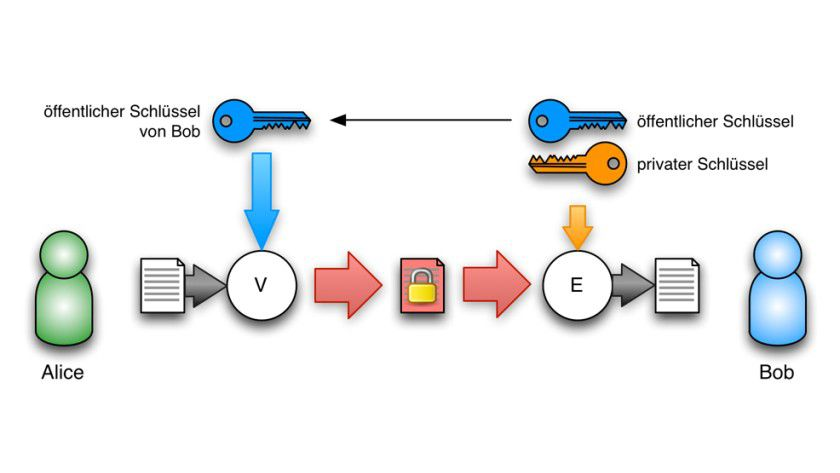
\includegraphics[width=12cm]{gfx/asymmetrisch.jpg}
	\caption{(V) Verschlüsseln\\(E) Entschlüsseln}
\end{figure}
\newpage
%--------------------------------------------------

\section{Beispiele zu Asymmetrischer Verschlüsselung}